% \documentclass{article}
% \usepackage[utf8]{inputenc}
% \begin{document}
% (Type your content here.)
% \end{document}
%%%
%%%  
%%%  
%%%
%%%
%%%              
%%%
%% pacotes não necessariamente necessários
\documentclass[a4paper,12pt]{article}
\usepackage[T1]{fontenc} 
\usepackage[brazil]{babel}    
\usepackage[utf8]{inputenc}
\usepackage{ae}
\usepackage{pgf,xcolor,pgfarrows,pgfnodes,pgfautomata,pgfheaps,pgfshade}
\usepackage{graphicx,url,geometry}
\usepackage{amsmath,amssymb}
\usepackage{fancyvrb}
\usepackage{fancyhdr}
\usepackage{float}
\usepackage{multirow}
\usepackage{enumerate}
\graphicspath{{./Figuras/}}    
\definecolor{shadecolor}{rgb}{0.8,0.8,0.8}
\usepackage{colortbl}
\DeclareMathSizes{11}{11}{11}{11}
\usepackage{indentfirst} 

%%\usepackage{bbm}   
%%\usepackage{color}
%%\usepackage{indentfirst}
%%\usepackage{lineno} %para adicionar linhas, usar com \linenumbers
%%\usepackage{listings}
\usepackage[pdftex,% 
                    pdfauthor = {Rafael Cardoso Pereira},pdftitle = {titulo},%
                    pdftoolbar=false,pdfmenubar=false,%
                    pdffitwindow=false,
                    hidelinks]{hyperref}

\geometry{a4paper, left=1in, right=1in, top=0.5in, bottom=1.0in}

\pagestyle{fancyplain}

\pdfminorversion=4

%FAZ EDICOES AQUI (somente no conteudo que esta entre entre as ultimas  chaves de cada linha!!!)
\newcommand{\universidade}{UFRN}
\newcommand{\centro}{Centro de Tecnologia}
\newcommand{\departamento}{Departamento de Engenharia Elétrica}
\newcommand{\aval}{RELATÓRIO LABORATORIAL}
\newcommand{\professor}{Rafael Cardoso}
\newcommand{\data}{26/03/2018}
\newcommand{\disciplina}{ELE0701 - ELETRÔNICA}
\newcommand{\compA}{Josiel Patricio Pereira de Oliveira}
\newcommand{\matrA}{20180010388}
\newcommand{\compB}{Wesley Wagner Varela Souza}
\newcommand{\matrB}{2015012638}
% \newcommand{\compC}{Cassio Fonseca Baracho}
% \newcommand{\matrC}{20170149830}

%ATE AQUI !!!

\begin{document}

	\pagestyle{empty}
	\begin{tabular}{ll}
	\multirow{3}{*}{
\includegraphics[width=0.2\linewidth]{UFRN.pdf}} & \universidade\\
		& \centro\\
		& \departamento\\
	\end{tabular}
	\begin{center}
	
	 	\vspace{0pt}

		\vspace{24pt}
		\LARGE \textbf{\aval}
		
	\end{center}
	
	\vspace{24pt}
	
	\begin{tabular}{ |l|p{12cm}| }
		
		\hline
		\multicolumn{2}{|c|}{\textbf{Dados de Identificação}} \\
			\hline
		Comp. curricular:        &    \disciplina          \\
		\hline
		Data do exper.:         &    \data           \\
	\hline
	Componentes:         & \begin{tabular}{r|l}
	\matrA & \compA\\
	\matrB & \compB\\
% 	\matrC & \compC\\
	\end{tabular} \\
	\hline
	\end{tabular}
	
	\vspace{14pt}
%%% FINAL DA CAPA

\section{Introdução} 
Relatório de aula prática com amplificadores operacionais. Serão montados circuitos retificação valores teóricos encontrados a partir da aplicação dos conceitos apresentados em sala com resultados obtidos em medições de circuitos reais.
Um amplificador operacional ou amp op é um amplificador com ganho muito elevado, tendo dois terminais de entrada: um designado por terminal inversor(-) e o outro identificado por terminal não inversor(+) . A tensão de saída é a diferença entre as entradas (+) e (-) , multiplicado pelo ganho em malha aberta. Devido ao alto ganho, quando usado em malha aberta são circuitos geralmente chamados de comparadores. O simbolo elétrico e detalhes dos terminais comuns em amp op são  mostrados na figura \ref{pinout}.

O amplificador operacional ideal tem um ganho infinito em malha aberta, largura de banda infinita, impedância de entrada infinita, impedância de saída nula e nenhum ruído, assim como offset de entrada é zero (exatamente 0 V na saída quando as duas entradas forem exatamente iguais) e nenhuma interferência térmica. Os circuitos integrados de amp ops utilizando MOSFETs são os que mais se aproximam destes valores ideais em limites de largura de banda.

\begin{figure}[!ht]
\label{pinout}
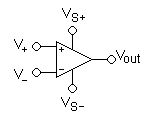
\includegraphics[width=0.5\linewidth]{pinout.png}
\caption{símbolo elétrico e detalhes da pinagem comum entre amplificadores operacionais}
(V+) entrada não-inversora; (V-) entrada inversora; (Vout) saída (VS+) alimentação positiva; (VS-) alimentação negativa
\end{figure}

Os pinos de alimentação (VS+ e VS- podem ser nomeados de diferentes formas. Ver pinos de alimentação dos CIs. Para amp ops baseados em tecnologia FET, o positivo, ou alimentação de dreno comum é chamada do VDD e o negativo, ou alimentação de fonte comum é chamado de VSS. Para amp ops baseados em TJB (BJT), o pino VS+ torna-se VCC e o pino VS- torna-se VEE. Eles são muitas vezes chamados VCC+ e VCC-, ou mesmo V+ e V-, no caso de as entradas serem nomeadas diferentemente, a função permanecerá a mesma. Muitas vezes estes pinos são retirados dos esquemas elétricos para uma maior clareza, e a configuração de alimentação é dada ou previsível através do circuito.
%Na introdução deve haver uma contextualização do assunto abordado no documento, por exemplo: se o documento for um relatório a respeito de uma aula laboratorial sobre amplificadores de tensão, deve-se fazer uma explanação sobre o contexto em que os amplificadores de tensão estão inseridos, sua importância, onde são utilizados, etc...\\
%A introdução também deve conter um breve explicação dos conhecimentos necessários para se entender o assunto que será abordado nas demais seções.
%Falar de diodos retificação e fabricação de fontes 



\newpage
\section{Metodologia}
%Na metodologia deve ser feita uma explicação de toda a base teórica necessária no desenvolver do assunto do relatório. Por exemplo: se o documento for um relatório a respeito de uma aula laboratorial sobre amplificadores de tensão, na metodologia deve haver uma breve explicação sobre amplificadores de tensão e seu funcionamento básico.

Foram montados os circuitos de acordo com os esquemas propostos no material de preparação para o laboratório conforme imagens abaixo:

\begin{figure}[!ht]
\label{meia}
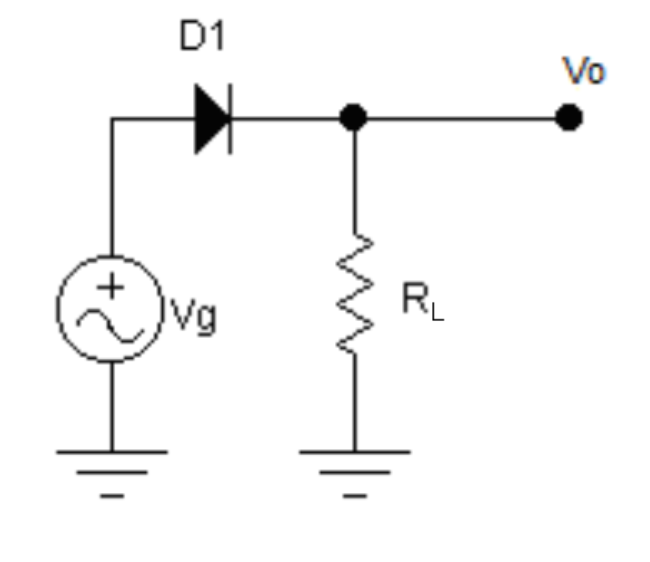
\includegraphics[width=0.5\linewidth]{meia.png}
\caption{Circuito de retificação de meia onda}
\end{figure}

\begin{figure}[!ht]
\label{completa}
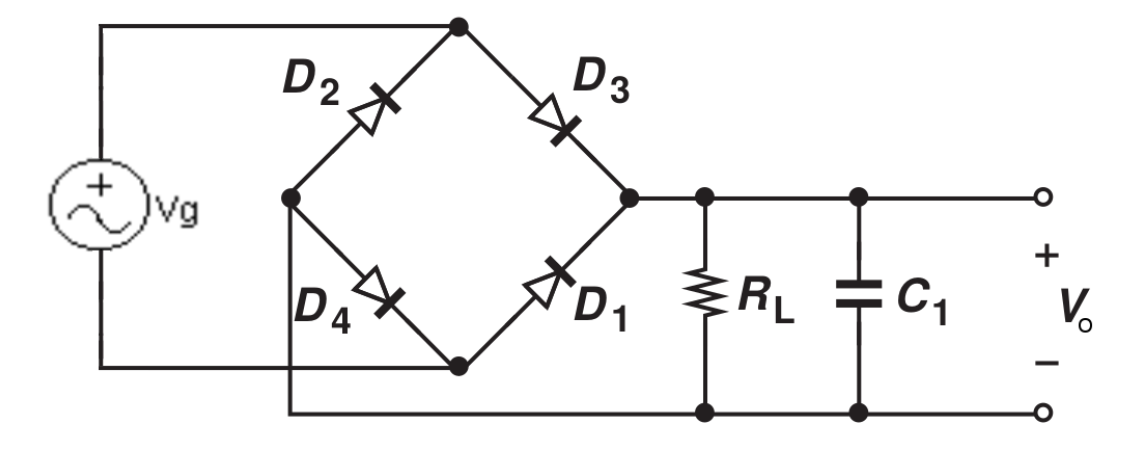
\includegraphics[width=0.5\linewidth]{completa.png}
\caption{Circuito de retificação de onda completa}

\end{figure}

Após a montagem do circuito foram realizadas medições para comparação com os valores calculados previamente.

Para os circuitos adotamos o modelo de tensão constante no qual VD$_{on}$ apresenta um valor de 0,7V. 

Esses circuitos são importantes tanto pra validar os métodos utilizados na aplicação dos cálculos das tensões e correntes adotando os modelos matemáticos apresentados em sala: modelo ideal associa o diodo a uma chave ,conduzindo apenas no sentido convencional anodo->catodo; modelo de tensão, parecido com o modelo ideal a menos de uma fonte CC em série com a chave para representar a tensão VD$_{on}$; modelo para pequenos sinais modelo exponencial.
Para fins de confrontação das análises feitas no circuito real, cujos dados apresentados a seguir foram registrados por meio de um osciloscópio, será usado, para efeito de cálculo para estimativa de valores, o modelo tensão constante.

\subsection{Materiais}

%Deve conter uma listagem dos materiais utilizados ao se desenvolver alguma aplicação prática.
\begin{itemize}
\item 1 x Resistor de 10k$\Omega$*
\item 1 x Resistor de 68k$\Omega$
\item 4 x Diodos 1N4148

\end{itemize}

* O diodo Zener não estava com o código legível. 


\section{Discussões}
 Durante a montagem dos circuitos, as realizações das devidas medições foram registradas em forma de imagens retiradas diretamente da tela do instrumento de medição registrando os valores bem como a forma de onda após a retificação. Essas imagens serão mostradas na subseção adiante.
 Também aparecerem alguns mal-contatos em decorrência dos equipamentos utilizados.
 Houve o reinicio do osciloscópio durante um processo de medição, o qual não comprometeu o andamento da experiência.
 Ocorreu também o problema da falta de legibilidade na leitura do código do zener, porém pelos resultados apresentados na resposta do circuito julgamos ser de um valor maior que 4,5V em virtude de sua inclusão no circuito não causar alterações significativas nos valores de V$_o$

\section{Resultados}
\subsection{Imagens das medidas}

 A primeira imagem representa as medições para o circuito de retificação de meia onda fig. \ref{meia}. cujo valores da fonte são: Vg=5V$_p$, 150Hz.
Como observado na fig.\ref{meia-osc} os valores são próximos do esperado. V$_o$=V$_p$-V$_{on}$. Aplicando o modelo de tensão constante para VD$_{on}$=0,7V, temos V$_{o}$=5-0,7. 

\begin{figure}[!ht]

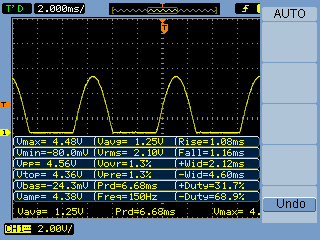
\includegraphics[width=0.5\linewidth]{0011.png}
\caption{Medição do circuito de retificação de meia onda}
\label{meia-osc}
\end{figure} 

%Nesta seção deve constar uma explanação de como o assunto do relatório foi desenvolvido. Por exemplo: se o documento for um relatório a respeito de uma aula laboratorial sobre amplificadores de tensão, no desenvolvimento deve constar uma explicação detalhada do que foi feito durante a aula.


\begin{figure}[!ht]

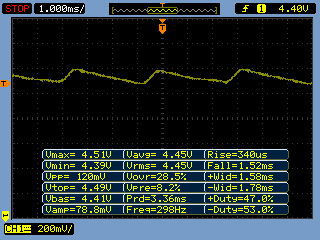
\includegraphics[width=0.5\linewidth]{0021.png}
\caption{Medição do circuito de retificação de onda completa com um capacitor}
\label{completa-1-osc}
\end{figure} 

\begin{figure}[!ht]
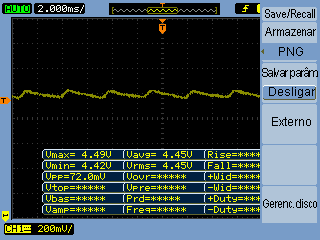
\includegraphics[width=0.5\linewidth]{0022.png}
\caption{Medição do circuito de retificação de onda completa com dois capacitores}
\label{completa-2-osc}
\end{figure} 

\begin{figure}[!ht]
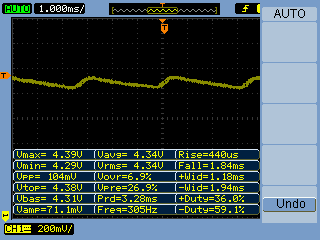
\includegraphics[width=0.5\linewidth]{0023.png}
\caption{Medição do circuito de retificação de onda completa com um capacitore diodo zener}
\label{completa-3-osc}
\end{figure} 

\begin{figure}[!ht]
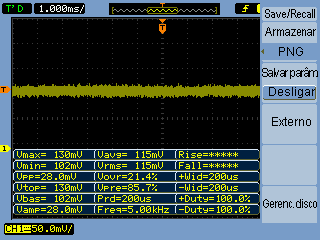
\includegraphics[width=0.5\linewidth]{0024.png}
\caption{Medição do circuito de retificação de onda completa com um capacitor e diodo zener e com tensão na fonte de Vg=1V$_p$}
\label{completa-4-osc}
\end{figure} 
\pagebreak

\section{Conclusões}
A Experiência foi muita válida pois mostrou como os valores reais podem ser aproximados com uma boa precisão tendo como base o modelo de tensão constante. Foi possível ver também o estado de não condução do circuito quando aplicado uma tensão menos que 2VD$_{on}$ como visto na fig.\ref{completa-4-osc}. As tesões com retificação em onda completa figs. \ref{completa-1-osc} e \ref{completa-2-osc} mostram como o aumento do valor da capacitância influênciou no valor do \textit{ripple}.


%vmax = v_p - v_d_o_n
%vmed = \frac{v_p - v_d_o_n}{\pi}
%vmin = 0
%T = \frac{1}{f}

% A seção de resultados deve conter os resultados esperados para a aplicação, bem como os resultados obtidos na prática. Deve conter resultados teóricos obtidos através de cálculos ou simulações e tabelas ou gráficos com comparações entre os resultados práticos com os resultados teóricos.

%\section{Conclusões}

% Aqui deve ser feita uma recapitulação do que foi feito e uma análise dos resultados obtidos. Por fim deve conter uma avaliação da qualidade do trabalho e o que poderia ter sido feito para melhorar.

\pagebreak
%% Essa seção não é necessária no relatório final, serve apenas como apoio didático
% \section*{Notas gerais (seção não obrigatória)}

% \begin{itemize}
% \item Todas as figuras e tabelas constantes no documento devem ser referenciadas no texto (isso pode ser feito utilizando-se \verb$\cite{fig:label}$ no Latex).
% \item Deve-se realizar pelo menos uma revisão do documento para evitar possíveis erros de ortografia, coesão e coerência textual.
% \item Todo e qualquer assunto presente no documento que não for de autoria dos alunos deve ser referenciado.
% \item Todos os relatórios devem conter bibliografia.
% \item O relatório final deve ser entregue em formato .pdf (Deve ser exportado para pdf caso seja feito utilizando-se o {\em Microsoft Word}).
% \item A seção {\bf Notas gerais} não é necessária no relatório final, servindo apenas como apoio didático na elaboração do mesmo.
% \end{itemize}

%% para inserção de figuras o seguinte código pode ser utilizado
%\begin{figure}[h!]
%       \centering
%        \includegraphics[height = 6 cm,width=10 cm]{../imagem/Img01.png}      
%        \caption{\protect\label{fig:label} legenda}
%\end{figure}

%% para inserção de tabelas o seguinte código pode ser utilizado
% \begin{table}
%\begin{tabular}{ccc}
%\\ $\tau_{o} = \frac{10}{22,4} = 45\%$ \\
%\\ $\tau_{o} = \frac{4,2}{22,4} = 19\%$ \\
%\\ $\tau_{o} = \frac{17,6}{22,4} = 80\%$ \\
%\end{tabular}
%\caption{\protect\label{tab:label} legenda}
%\end{table}

\pagebreak
\newpage


%%% BIBLIOGRAFIA

\end{document}
